\ifdefined\XeTeXversion
\documentclass[a4paper,11pt,xelatex,ja=standard]{bxjsarticle}
\else
\documentclass[a4paper,11pt,platex,dvipdfmx,ja=standard]{bxjsarticle}
\fi
\geometry{reset,top=20mm,bottom=25mm,left=20mm,right=20mm}
\usepackage{amsmath,amssymb,booktabs,longtable,graphicx,float}
\ifdefined\XeTeXversion
\setCJKmainfont{HaranoAjiMincho-Regular.otf}
\setCJKsansfont{HaranoAjiGothic-Medium.otf}
\else
\usepackage[haranoaji]{pxchfon}
\fi
\setlength{\abovedisplayskip}{6pt}
\setlength{\belowdisplayskip}{6pt}
\title{\vspace{-20mm}今月の進捗報告\\[0.5em]\large EMS最適化手法の比較研究\\LP・MILP・DPの比較と最適化期間による運用の違い}
\author{神戸大学大学院システム情報学研究科 修士1年\\山崎博之}
\date{2026年10月}
\begin{document}
\maketitle

\section{背景と目的}
太陽光発電（PV）と蓄電池を備えたエネルギーマネジメントシステム（EMS）について，電気料金を最小化する充放電計画を対象とする．10月は，論文作成に向けて共通の数理モデルを整理し，線形計画法（LP），混合整数線形計画法（MILP），動的計画法（DP）の費用と計算時間を比較した．さらに，最適化期間と時間間隔を変え，同じ1日の運用がどのように異なるかを確認した．

本報告は，10月2日・8日・16日の週次報告をまとめたものである．数値は10月16日報告の結果を用い，それ以前の結果と重複して集計していない．

\section{検証条件}
需要・PV・蓄電池1台・系統買電からなる共通モデルを用いた．入力は北海道十勝地方の施設における2025年の需要電力量とPV発電量の実測値である．30分ごとの電力量［kWh］を各区間の平均電力［kW］へ換算し，60分の条件では隣接する30分値2点の平均電力を用いた．この集約では総電力量を保存する．

\begin{table}[H]
    \centering
    \small
    \caption{期間・時間刻みの比較条件}
    \label{tab:conditions}
    \begin{tabular}{lccc}
        \toprule
        条件      & 対象期間（2025年） & 時間刻み & 区間数   \\
        \midrule
        1日・30分  & 7月22日       & 30分  & 48    \\
        7日・30分  & 7月22～28日    & 30分  & 336   \\
        30日・30分 & 7月22日～8月20日 & 30分  & 1,440 \\
        7日・60分  & 7月22～28日    & 60分  & 168   \\
        \bottomrule
    \end{tabular}
\end{table}

\begin{table}[H]
    \centering
    \small
    \caption{電気料金と蓄電池の計算条件}
    \label{tab:system-conditions}
    \begin{tabular}{p{46mm}p{91mm}}
        \toprule
        項目        & 設定             \\
        \midrule
        買電単価      & 21.51\,円/kWh   \\
        月額基本料金単価  & 2,829.60\,円/kW \\
        力率補正係数    & 0.85           \\
        蓄電池定格容量   & 860\,kWh       \\
        最大充電・放電電力 & 400\,kW        \\
        充電・放電効率   & 0.98           \\
        運用SOC範囲   & 定格容量の5～95\%    \\
        初期・終端SOC  & 定格容量の50\%      \\
        \bottomrule
    \end{tabular}
\end{table}


各条件についてLP，MILP，SOCを19，37，73，145点に離散化したDPを比較した．各手法は事前準備後に4回実行し，求解の打切り設定を600秒とした．費用と計算時間は成功試行のみの平均値であり，時間切れの試行は平均に含めない．

\clearpage
\begingroup
\small
\section{運用手法}
\subsection{目的関数}
時刻区間を$k=0,1,\ldots,K-1$，1区間の幅を$\Delta t$［h］とする．$d_k$は需要電力，$g^{\mathrm{P1}}_k$は利用可能なPV電力，$p^{\mathrm{BY}}_k$は買電単価であり，いずれも既知とする．決定変数$s^{\mathrm{BY}}_k$は買電電力，$s^{\mathrm{BY}}_{\mathrm{MAX}}$は対象期間内の最大買電電力を表す．目的関数は，基本料金相当額と電力量料金の合計を最小化する．
\begin{equation}
    \text{Minimize}\quad C_{\mathrm{total}}
    = w_{\mathrm{basic}}s^{\mathrm{BY}}_{\mathrm{MAX}}
    + \sum_{k=0}^{K-1}p^{\mathrm{BY}}_k s^{\mathrm{BY}}_k\Delta t
    \label{eq:objective}
\end{equation}
買電単価は全時刻で$p^{\mathrm{BY}}_k=21.51$［円/kWh］とした．基本料金係数$w_{\mathrm{basic}}$［円/kW］には，年間単価を対象期間の時間数$K\Delta t$に比例させた次式を用いる．
\begin{equation}
    w_{\mathrm{basic}}
    = (2{,}829.60\times0.85\times12)
    \frac{K\Delta t}{8{,}760}
    \label{eq:basic-weight}
\end{equation}
ここで，8,760は2025年の1年間の時間数（365日$\times$24時間）である．
この基本料金は，実際の過去12か月を参照する月別契約電力ではなく，比較対象期間の最大買電電力を使った代理的な評価である．

\subsection{制約条件}
以下の式は，各区間$k=0,\ldots,K-1$に適用する．$g^{\mathrm{P2}}_k$を利用するPV電力，$x^{\mathrm{FC1}}_k$と$x^{\mathrm{FC2}}_k$を電池の外部側・内部側の充電電力，$x^{\mathrm{FD1}}_k$と$x^{\mathrm{FD2}}_k$を内部側・外部側の放電電力，$b^{\mathrm{F}}_k$を区間境界$k$の蓄電量［kWh］とする．

\begin{enumerate}
    \item \textbf{電力需給バランスと変換効率}：
          \begin{equation}
              g^{\mathrm{P2}}_k+s^{\mathrm{BY}}_k+x^{\mathrm{FD2}}_k
              =d_k+x^{\mathrm{FC1}}_k \label{eq:balance}
          \end{equation}
          \begin{equation}
              x^{\mathrm{FC2}}_k=\alpha_{\mathrm c}x^{\mathrm{FC1}}_k
              \label{eq:charge-efficiency}
          \end{equation}
          \begin{equation}
              x^{\mathrm{FD2}}_k=\alpha_{\mathrm d}x^{\mathrm{FD1}}_k
              \label{eq:discharge-efficiency}
          \end{equation}
          充電・放電の変換効率はそれぞれ$\alpha_{\mathrm c}=\alpha_{\mathrm d}=0.98$とする．

    \item \textbf{PV利用量と買電電力}：売電は行わない．
          \begin{equation}
              0\leq g^{\mathrm{P2}}_k\leq g^{\mathrm{P1}}_k,\qquad
              s^{\mathrm{BY}}_k\geq0 \label{eq:pv-buy}
          \end{equation}

    \item \textbf{蓄電量の遷移，範囲，境界条件}：定格容量を$C$とする．
          \begin{align}
              b^{\mathrm{F}}_{k+1}
                               & =b^{\mathrm{F}}_k+
              (x^{\mathrm{FC2}}_k-x^{\mathrm{FD1}}_k)\Delta t
              \label{eq:soc-update}                    \\
              0.05C            & \leq b^{\mathrm{F}}_j
              \leq0.95C
              \quad(j=0,\ldots,K) \label{eq:soc-range} \\
              b^{\mathrm{F}}_0 & =b^{\mathrm{F}}_K
              =0.50C=430\ \mathrm{kWh} \label{eq:soc-boundary}
          \end{align}
          蓄電量は区間の両端に定義するため，$K$区間に対して$K+1$点である．

    \item \textbf{充放電出力と排他制約}：MILPでは二値変数$z_k\in\{0,1\}$を用い，同時充放電を明示的に禁止する．
          \begin{equation}
              0\leq x^{\mathrm{FC2}}_k\leq P^{\mathrm{FC}}_{\mathrm{max}}z_k,
              \qquad
              0\leq x^{\mathrm{FD1}}_k\leq P^{\mathrm{FD}}_{\mathrm{max}}(1-z_k)
              \label{eq:exclusive}
          \end{equation}
          LPでは$z_k$と排他制約を除き，$0\leq x^{\mathrm{FC2}}_k\leq P^{\mathrm{FC}}_{\mathrm{max}}$，$0\leq x^{\mathrm{FD1}}_k\leq P^{\mathrm{FD}}_{\mathrm{max}}$を課す．DPでは蓄電量の増減方向から充電と放電のいずれか一方を選ぶ．

    \item \textbf{最大買電電力}：
          \begin{equation}
              0\leq s^{\mathrm{BY}}_k\leq s^{\mathrm{BY}}_{\mathrm{MAX}},
              \qquad s^{\mathrm{BY}}_{\mathrm{MAX}}\geq0
              \label{eq:max-buy}
          \end{equation}
          最適解では期間内の買電電力の最大値と一致する．
\end{enumerate}

DPのSOC格子は5～95\%の範囲に19，37，73，145点を等間隔に配置し，初期・終端の50\%を厳密に含める．各SOCについて累積電力量料金とその時点までの最大買電電力の非劣ラベルを保持し，終端で式(\ref{eq:objective})を評価する．このため，DPもLP・MILPと同じ基本料金と電力量料金を対象とする．

\endgroup

\clearpage
\section{計算結果}
10月8日に報告した比較実験192件は168件成功，24件時間切れ，失敗0件であった．3日計画の追加実験は，これらと分けて第5節に示す．

\subsection{最適化期間と時間間隔}
2025年7月22日を開始日とし，1日・7日・30日の計画を比較した．表\ref{tab:period}に，各手法の費用と計算時間を示す．成功数が0の条件は4回とも時間切れであり，費用と計算時間を欠測としている．

\begingroup
\small
\setlength{\tabcolsep}{3pt}
\begin{longtable}{llrrr}
    \caption{期間・時間刻み別の費用と処理時間（各手法4回）}\label{tab:period} \\
    \toprule
    条件      & 手法     & 成功/4 & 費用平均値 [円] & 時間平均値 [秒]     \\
    \midrule
    \endfirsthead
    \toprule
    条件      & 手法     & 成功/4 & 費用平均値 [円] & 時間平均値 [秒]     \\
    \midrule
    \endhead
    1日・30分  & LP     & 4    & 57,869    & 0.02          \\
            & MILP   & 4    & 57,869    & 0.02          \\
            & DP-19  & 4    & 60,972    & 0.06          \\
            & DP-37  & 4    & 59,650    & 0.51          \\
            & DP-73  & 4    & 58,776    & 3.96          \\
            & DP-145 & 4    & 58,307    & 31.08         \\
    \midrule
    7日・30分  & LP     & 4    & 545,929   & 0.07          \\
            & MILP   & 4    & 545,929   & 0.47          \\
            & DP-19  & 4    & 565,887   & 1.40          \\
            & DP-37  & 4    & 557,292   & 12.19         \\
            & DP-73  & 4    & 551,850   & 107.04        \\
            & DP-145 & 0    & --        & --            \\
    \midrule
    30日・30分 & LP     & 4    & 2,441,484 & 0.46          \\
            & MILP   & 4    & 2,441,484 & 2.01          \\
            & DP-19  & 4    & 2,542,031 & 7.85          \\
            & DP-37  & 4    & 2,495,660 & 75.50         \\
            & DP-73  & 0    & --        & --            \\
            & DP-145 & 0    & --        & --            \\
    \midrule
    7日・60分  & LP     & 4    & 545,625   & 0.03          \\
            & MILP   & 4    & 545,625   & 0.23          \\
            & DP-19  & 4    & 558,579   & 1.68          \\
            & DP-37  & 4    & 550,115   & 14.99         \\
            & DP-73  & 4    & 547,828   & 122.42        \\
            & DP-145 & 0    & --        & --            \\
    \bottomrule
\end{longtable}
\endgroup


LPとMILPは表\ref{tab:period}の全条件で4回とも成功し，表示した費用は一致した．30日・30分では，LPが0.46秒，MILPが2.01秒であった．DPはSOC格子を細かくすると費用がLPの結果に近づく一方，計算時間が増加した．1日・30分のDPは145点まで成功したが，7日・30分では145点，30日・30分では73点と145点が4回とも時間切れとなった．

これらの結果は，今回の実装と入力条件における比較である．LPで観測された同時充放電は0\,kWであったが，排他制約を省略しても常に同じ結果になることを示したものではない．

\clearpage
\subsection{異なる入力条件}
冬（1月14～20日），春（4月15～21日），夏（7月22～28日），秋（10月14～20日）の各1週間を30分間隔で比較した．いずれも2025年のデータであり，各季節から選んだ1週間の入力条件4例として扱う．

\begingroup
\small
\setlength{\tabcolsep}{3pt}
\begin{longtable}{llrrr}
    \caption{異なる入力条件4例の費用と処理時間（各1週間，30分刻み，各手法4回）}\label{tab:season} \\
    \toprule
    季節 & 手法     & 成功/4 & 費用平均値 [円] & 時間平均値 [秒]                      \\
    \midrule
    \endfirsthead
    \toprule
    季節 & 手法     & 成功/4 & 費用平均値 [円] & 時間平均値 [秒]                      \\
    \midrule
    \endhead
    冬  & LP     & 4    & 83,719    & 0.07                           \\
       & MILP   & 4    & 83,719    & 0.28                           \\
       & DP-19  & 4    & 153,161   & 0.16                           \\
       & DP-37  & 4    & 96,245    & 0.79                           \\
       & DP-73  & 4    & 89,601    & 10.03                          \\
       & DP-145 & 4    & 86,811    & 123.93                         \\
    \midrule
    春  & LP     & 4    & 191,774   & 0.07                           \\
       & MILP   & 4    & 191,774   & 0.17                           \\
       & DP-19  & 4    & 214,988   & 0.19                           \\
       & DP-37  & 4    & 204,237   & 2.44                           \\
       & DP-73  & 4    & 197,878   & 19.95                          \\
       & DP-145 & 4    & 194,230   & 213.77                         \\
    \midrule
    夏  & LP     & 4    & 545,929   & 0.07                           \\
       & MILP   & 4    & 545,929   & 0.48                           \\
       & DP-19  & 4    & 565,887   & 1.39                           \\
       & DP-37  & 4    & 557,292   & 12.00                          \\
       & DP-73  & 4    & 551,850   & 97.69                          \\
       & DP-145 & 0    & --        & --                             \\
    \midrule
    秋  & LP     & 4    & 283,335   & 0.09                           \\
       & MILP   & 4    & 283,335   & 0.42                           \\
       & DP-19  & 4    & 308,012   & 0.53                           \\
       & DP-37  & 4    & 293,684   & 6.74                           \\
       & DP-73  & 4    & 289,347   & 58.21                          \\
       & DP-145 & 0    & --        & --                             \\
    \bottomrule
\end{longtable}
\endgroup


LPとMILPの費用は4例とも一致した．DP-145は冬・春では4回とも成功したが，夏・秋では4回とも時間切れとなった．同じ1週間・30分間隔でも，入力条件によってDPの計算時間と成功数が異なった．各季節1週間の結果であるため，季節全体の傾向を結論づけるには対象期間を増やす必要がある．

\clearpage
\section{3日間の追加実験}
2025年7月22～24日の3日間について，30分間隔（144区間）と60分間隔（72区間）で比較した．その他の条件は表\ref{tab:system-conditions}と同じとし，各手法4回，求解の打切り設定600秒で実行した．60分値は隣接する30分値2点の平均電力とし，総電力量を保存した．

\begin{table}[H]
    \centering
    \caption{最適化期間3日の費用と処理時間（各手法4回）}
    \label{tab:three-days}
    \begin{tabular}{llrrr}
        \toprule
        時間間隔 & 手法     & 成功/4 & 費用平均値 [円] & 時間平均値 [秒] \\
        \midrule
        30分  & LP     & 4    & 205,002   & 0.03      \\
             & MILP   & 4    & 205,002   & 0.18      \\
             & DP-19  & 4    & 215,614   & 0.70      \\
             & DP-37  & 4    & 208,815   & 5.88      \\
             & DP-73  & 4    & 207,702   & 40.31     \\
             & DP-145 & 1    & 206,091   & 447.64    \\
        \midrule
        60分  & LP     & 4    & 204,886   & 0.03      \\
             & MILP   & 4    & 204,886   & 0.06      \\
             & DP-19  & 4    & 209,958   & 0.74      \\
             & DP-37  & 4    & 207,605   & 5.62      \\
             & DP-73  & 4    & 206,449   & 40.83     \\
             & DP-145 & 2    & 205,338   & 451.69    \\
        \bottomrule
    \end{tabular}
\end{table}

この追加実験48件は43件成功，5件時間切れ，失敗0件であり，成功解はすべて独立評価に合格した．費用と時間は成功試行のみの平均値である．60分値との費用差には時間集約による問題条件の変化も含まれる．



3日計画でもLPとMILPの費用は一致した．DP-145の成功数は30分間隔で1回，60分間隔で2回であり，表の平均値はそれぞれの成功試行のみを対象とする．格子点数の多いDPでは，一部の試行が成功しても4回すべてが時間内に終了するとは限らなかった．

7日計画では，30分間隔のDP-73が107.04秒，60分間隔が122.42秒であった．時間間隔を粗くしても，DPの計算時間が必ず短くなるわけではない．また，30分値と60分値では総電力量を保存していても区間ごとの電力が変わるため，費用差を計算手法だけの差として解釈しない．

\clearpage
\section{最適化期間による1日の運用の違い}
LP・DP37点・DP73点の1日・7日・30日計画から，共通する2025年7月22日の運用を取り出した．各条件の1回目の保存済み結果を用いた．30日計画のDP73点は4回とも時間切れであり，運用図には表示していない．

\begin{figure}[H]
    \centering
    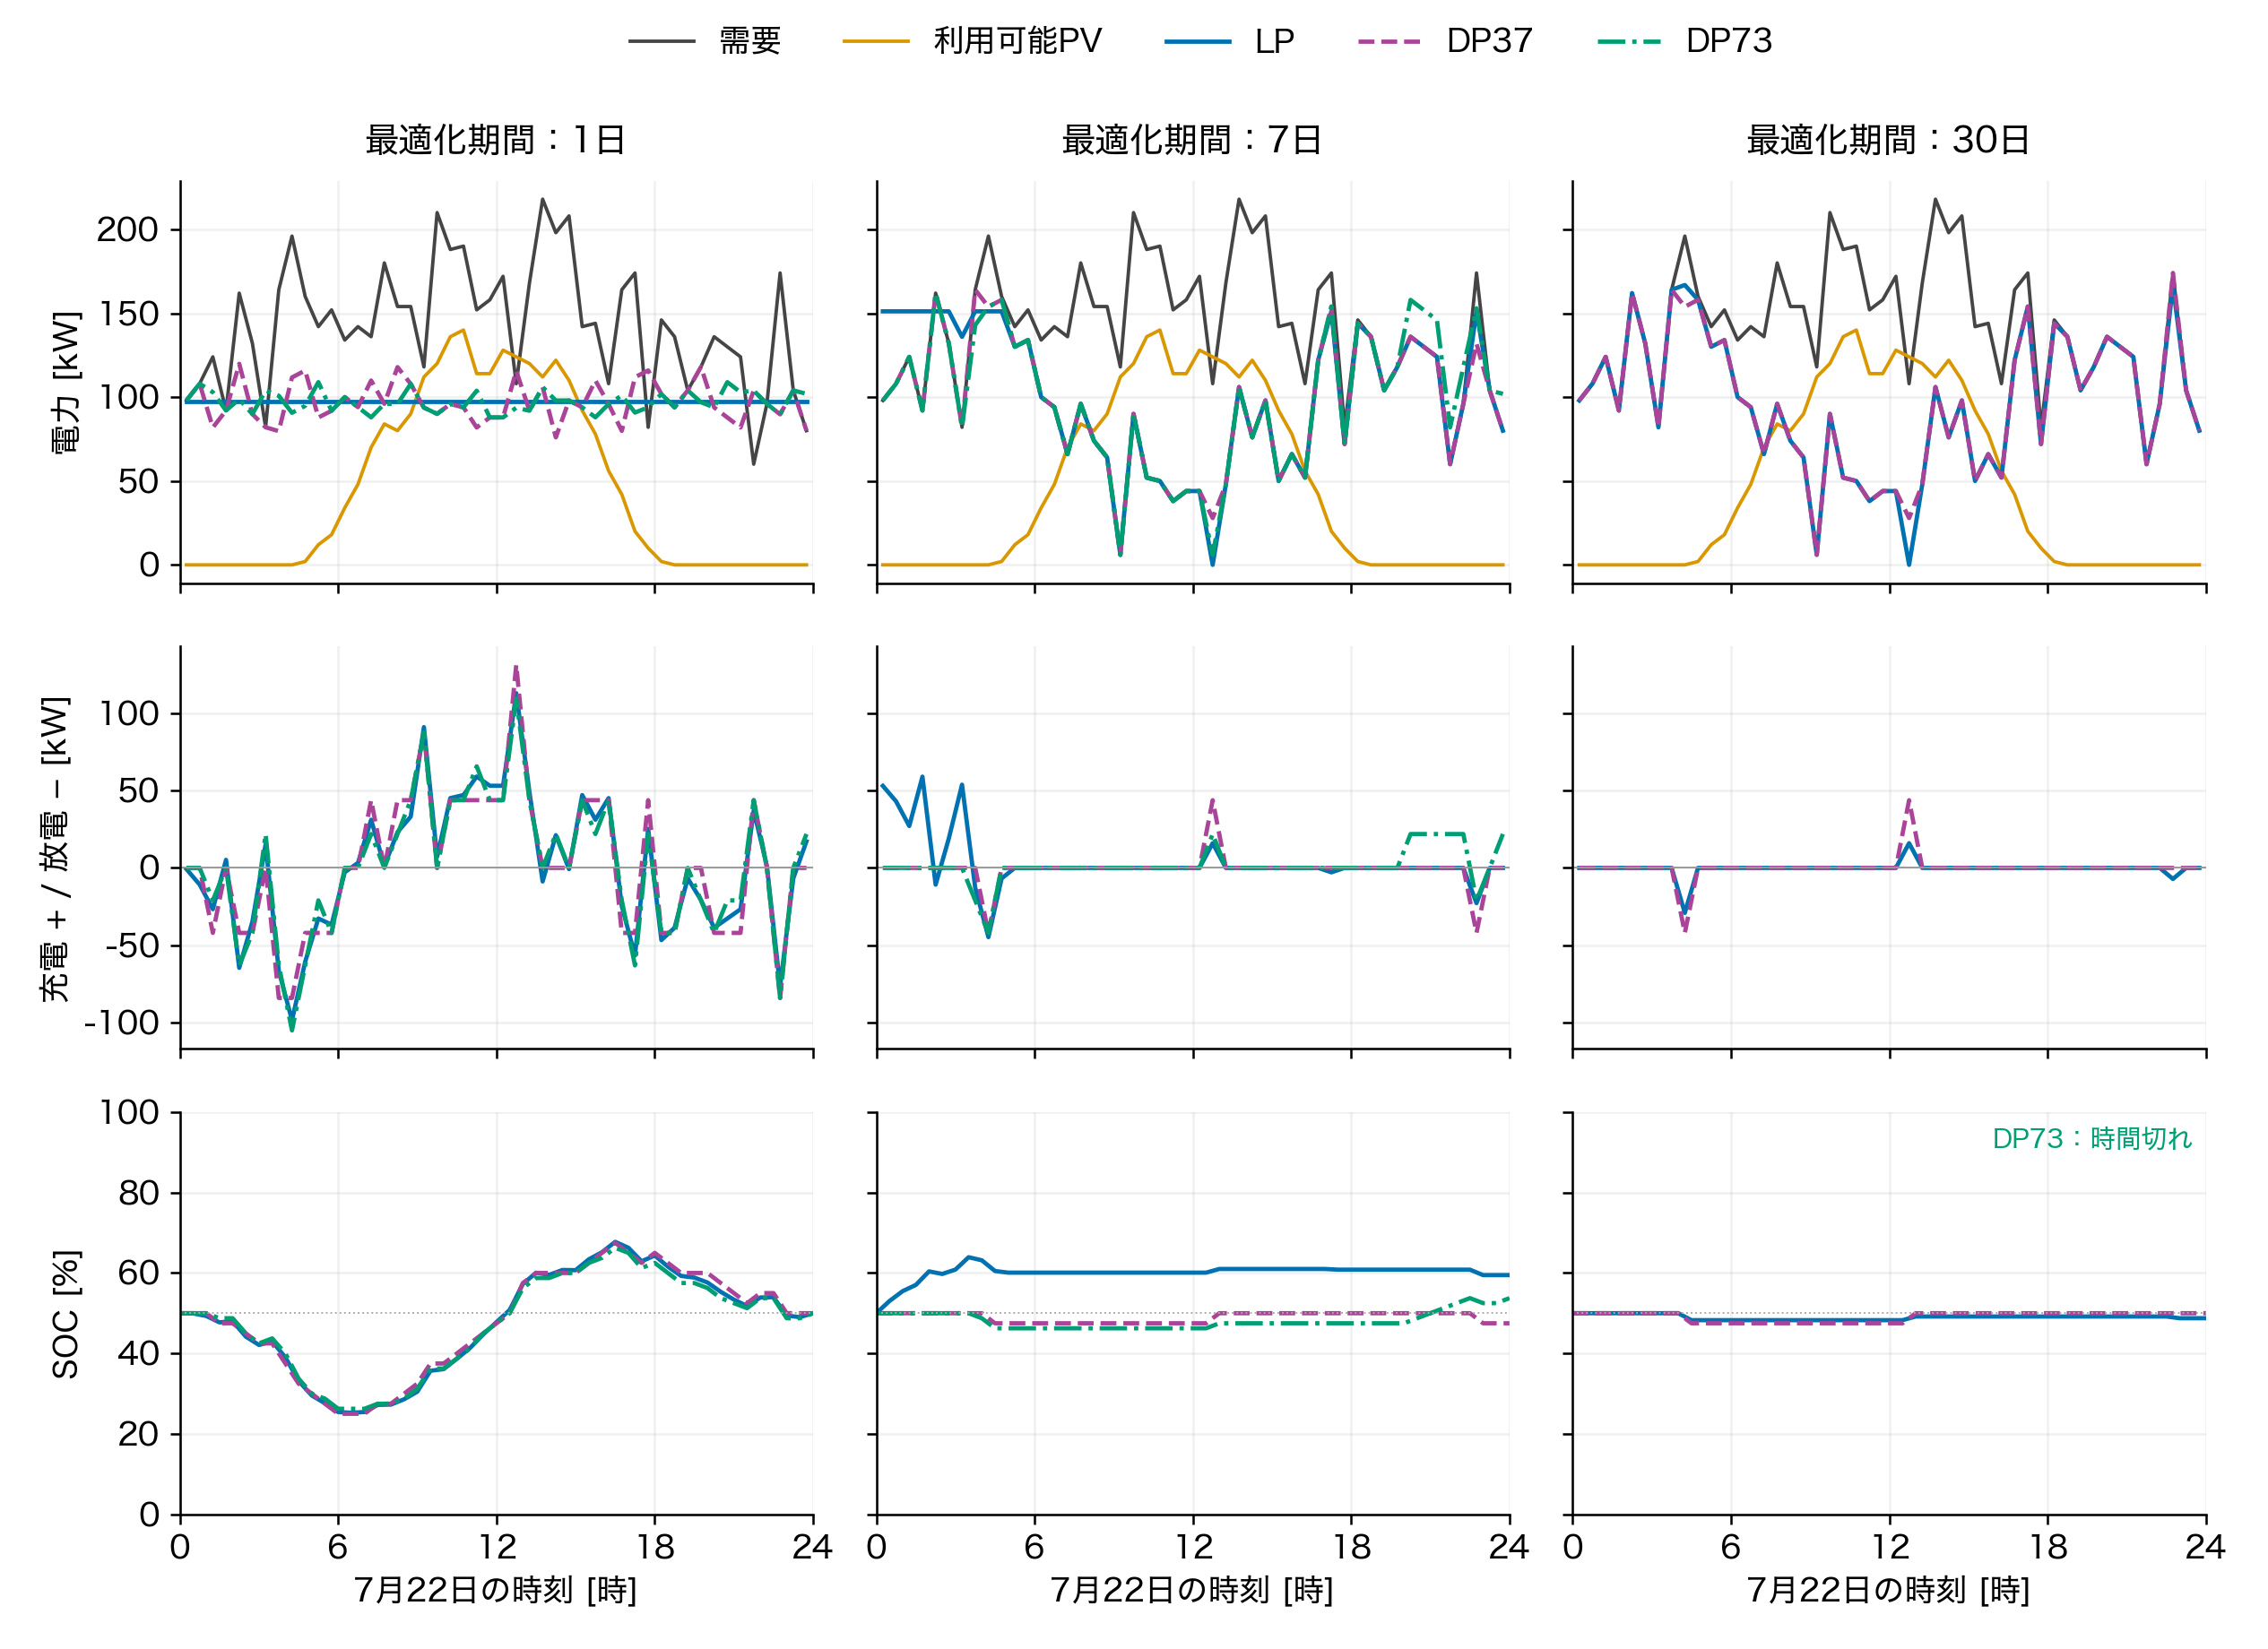
\includegraphics[width=0.85\textwidth]{../paper_method_comparison/figures/R1016_daily_operation.png}
    \caption{最適化期間別の7月22日の運用（30分刻み）．上段は需要・利用可能PV・各手法の買電，中段は外部側の充放電（充電を正，放電を負），下段はSOCを示す．電力は各区間の平均値を区間中央に置き，折れ線で結んだ．30日計画のDP73点は時間切れのため欠測とした．}
    \label{fig:daily-operation}
\end{figure}

\begin{table}[H]
    \centering
    \caption{7月22日の最大買電と24時のSOC（LP）}
    \begin{tabular}{lrr}
        \toprule
        最適化期間 & 当日の最大買電 [kW] & 当日24時のSOC [\%] \\
        \midrule
        1日    & 97.21        & 50.00          \\
        7日    & 151.13       & 59.47          \\
        30日   & 166.83       & 48.76          \\
        \bottomrule
    \end{tabular}
\end{table}



1日計画では7月23日0時が終端となるため，7月22日24時のSOCは50\%に固定される．7日・30日計画ではこの時点は期間の途中であり，表のSOCはそれぞれ59.47\%，48.76\%となった．同じ日のデータでも，対象期間と終端条件によって運用が異なることを確認した．各計画の目的関数は対象期間全体の費用であり，この表の当日最大買電だけで計画全体の優劣を判断することはできない．

\clearpage
\section{時間間隔による1日の運用の違い}
3日計画の各条件1回目のLP解から，7月22日の運用を取り出した．両条件の初期SOCは50\%であり，終端SOCは7月25日0時に50\%とする．固定単価では同費用の運用が複数あり得るため，図は各条件の最適解の一例である．

\begin{figure}[H]
    \centering
    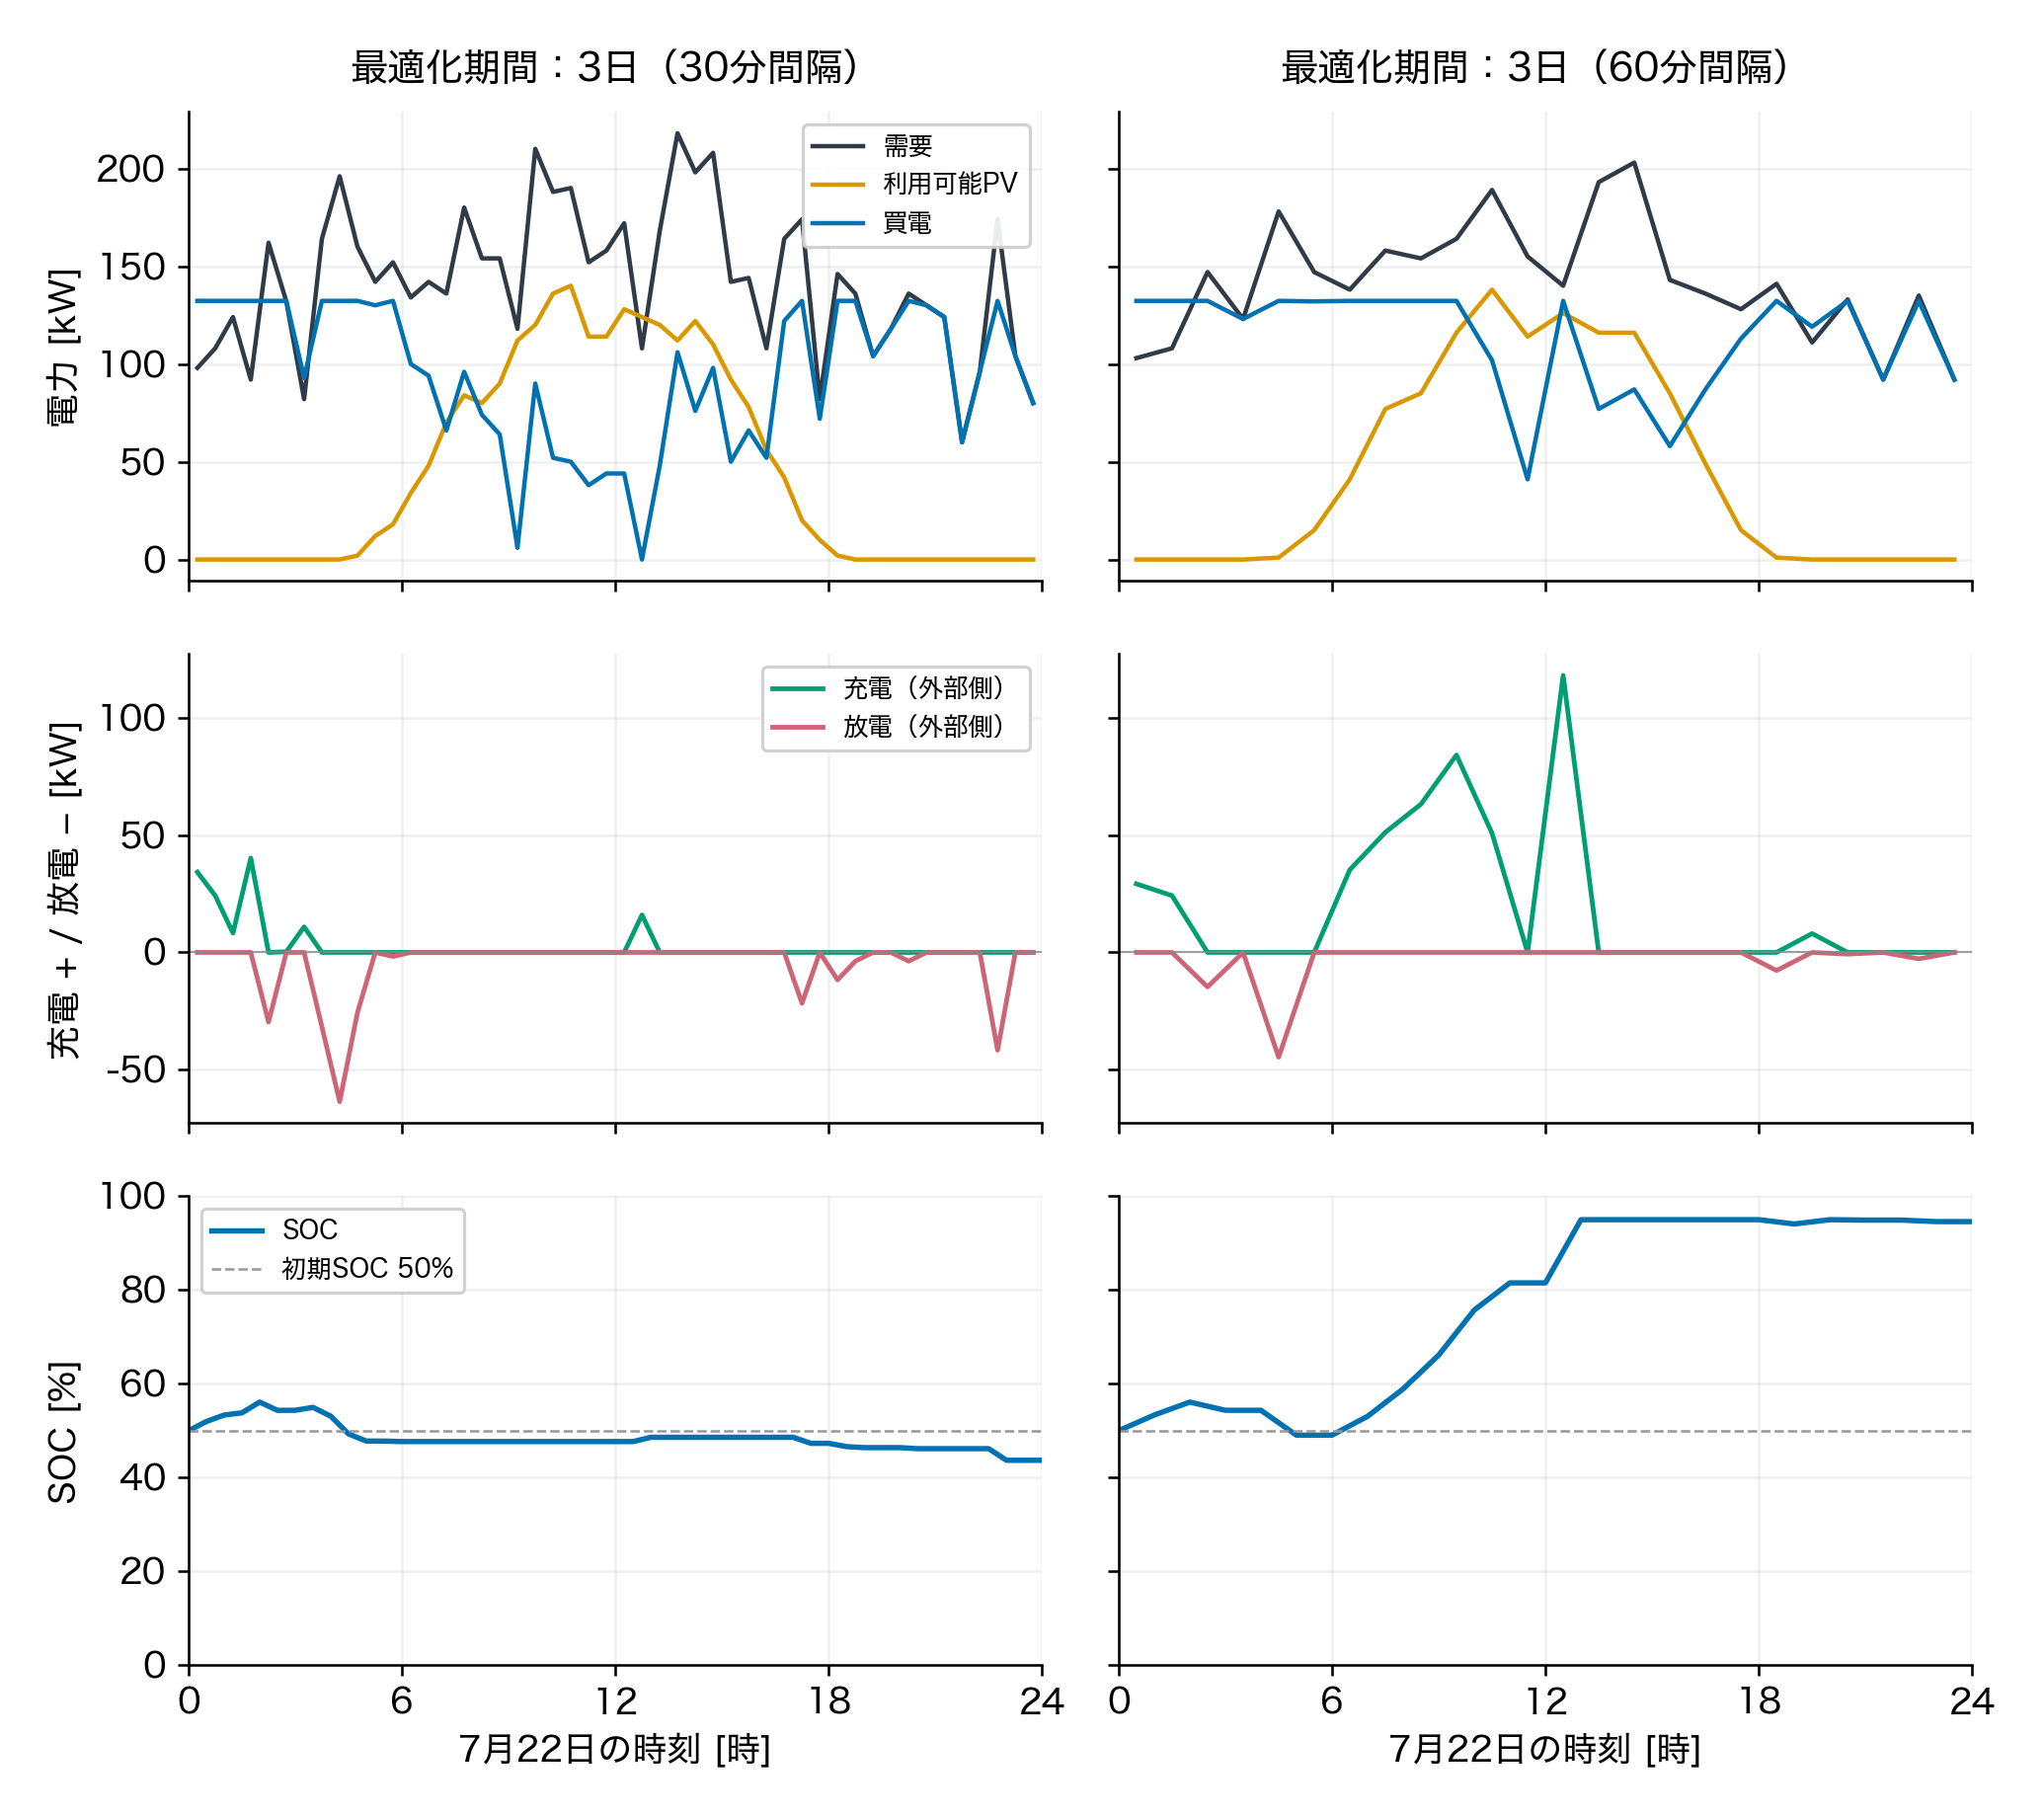
\includegraphics[width=0.72\textwidth]{../paper_method_comparison/figures/R1016_three_day_operation.png}
    \caption{最適化期間3日の7月22日の運用（LP）．電力は各区間の平均値を区間中央に置き，折れ線で結んだ．充放電は外部側で充電を正，放電を負とした．}
    \label{fig:three-day-operation}
\end{figure}


\section{今月の成果と今後の課題}
10月は，LP・MILP・DPを共通モデルで比較し，最適化期間，時間間隔，SOC格子点数，入力条件による費用と計算時間の違いを整理した．LPとMILPの費用は今回の比較条件で一致し，DPではSOC格子を細かくするほど費用がLPに近づく一方，長い計画期間や多い格子点数で時間切れが生じた．運用図からは，同じ1日でも計画期間と終端条件によって買電・充放電・SOCが異なることを確認した．

今後の検討課題として，DPの計算時間と時間切れに関係する条件の整理，入力期間を増やした比較，実際の月別契約電力を考慮した評価への拡張が挙げられる．今回の基本料金は期間内最大買電に基づく代理的な評価であり，7月に扱った過去12か月の月内最大買電を参照する年間評価とは区別する必要がある．
\end{document}
